\documentclass{article}
\usepackage[english]{babel}
\usepackage[utf8]{inputenc}
\usepackage[T1]{fontenc}

\usepackage{amsmath} % math stuff
\usepackage{amssymb} % math stuff
\usepackage{amsthm}  % math stuff
\usepackage{commath} % math stuff
\usepackage{relsize} % math stuff
\usepackage{caption} % caption stuff
\usepackage{fancyhdr} % custom headers
\usepackage{lastpage} % determine last page for the footer
\usepackage{extramarks} % headers and footers
\usepackage{graphicx} % images
\usepackage{listings} % code listings
\usepackage{courier} % courier font
\usepackage{enumerate}
\usepackage{enumitem}
\usepackage{mathtools}
\usepackage{titling}
\usepackage{float}
\usepackage{cite}

%tikz
\usepackage{tikz}

\title{Getting robots bored enough to move cubes}
\author{Julien Scholz}
\date{\today}

\begin{document}

\begin{titlepage}
    \centering
    
\includegraphics[width=10cm]{uhh_logo}\par
    \vspace{4\baselineskip}
    {\Large Bachelor thesis exposé\par}
    {\Huge \thetitle \par}
    \vspace{4\baselineskip}
    by\par
    {\Large \theauthor \par}
    \vspace{8\baselineskip}
    \vfill
    Thesis advisors:\par
    {\large Dr. Cornelius Weber, \par Muhammad Burhan Hafez}
\end{titlepage}

\tableofcontents

\section{Introduction}
Factory robots can perform complex tasks like car manufacturing extremely quickly and with millimeter accurate precision. However, outside of an assembly line setting, robots fail at even the most basic tasks due to the messiness of the real world. This is because predefined rules designed by humans fail to properly model the seemingly non-deterministic environment. Consequently, using artificial intelligence in the field of robotics has been an active area of research for many years.

The use of neural networks introduces additional issues. Useful data sets are rare, as the creation of large amounts of training labels would require an already existing solution to the problem. Alternatively, reinforcement learning can be used with a reward function that is arguably easier to define. While reinforcement learning has made large strides in recent times, two core issues persist, namely its sample inefficiency and its inability to train well with sparse rewards.

Sample efficiency is a metric which describes how well a reinforcement learning agent performs with relatively few state-action transition samples (i.e. little time spent exploring the environment). This metric is particularly important for robotics, because training with a real robot agent requires a realistic environment, is often high maintenance and is limited to real-time speed, while a simulation is often over-simplifying and computationally expensive. As such, an algorithm should make efficient use of the few examples it gets. To achieve this, model-based reinforcement learning can be used, that is, an algorithm that learns a model of the environment along with its action policy \cite{muzero}. The model can then be used for planning or to further train the policy \cite{muzero}.

When constructing a reward function, one must find a balance between accurately describing the goal with sparse rewards so as to not encourage unwanted behavior and placing additional rewards to reduce the amount of training necessary to converge. However, in robotics, it is very difficult to produce enough rewards to mitigate the enormous state and action spaces. There has been a new trend in reinforcement learning recently to use \textit{artificial curiosity} instead of (or in combination with) the traditional reward function \cite{curious}. With artificial curiosity, the agent is rewarded for exploring and discovering novel information of the environment. These rewards are generally less sparse and can lead to higher overall performance of the agent \cite{curious}.

\section{Prior work}
Prior work has already implemented a model-based reinforcement learning algorithm called \textit{MuZero} as well as several approaches to artificial curiosity. These algorithms will briefly be explained in the following sections.

\subsection{\textit{MuZero} algorithm}
\textit{MuZero} \cite{muzero} describes a model $\mu_\theta$ with parameters $\theta$ that is used to predict multiple quantities in a \textit{Markov decision process} (MDP). Internally, this is done at each time-step $t$ by first producing an internal state from past observations that does not necessarily have any semantic meaning. This internal state is then propagated forwards in time for each hypothetical time-step $k \in \{1, ..., K\}$. At each iteration, predictions of the policy $p$ and value $v$ can be made based on the current internal state. The following functions are used for this process:
\begin{enumerate}
    \item A \textit{representation} function $h_\theta$ that is used to produce the initial internal state $s^0 = h_{\theta}(o_1, ..., o_t)$ based on past observations.
    \item A \textit{dynamics} function that estimates subsequent immediate reward $r^k$ and internal state $s^k$ given a past internal state $s^{k-1}$ and an action $a^k$: \\ $(r^k, s^k) = g_\theta(s^{k-1}, a^k)$.
    \item A \textit{prediction} function $(p^k, v^k) = f_\theta(s^k)$ that computes policy $p^k$ and value $v^k$ for the virtual time-step $k$.
\end{enumerate}
\textit{Monte-Carlo tree search} (MCTS) can be used in combination with the dynamics function the to estimate a policy $\pi_t$.

With the help of a \textit{replay buffer}, the model can be trained by unrolling it for several time-steps and then propagating the error backwards through time so as to reduce it and improve predictions for future iterations.

A full visual representation of the aforementioned functions can be seen in figure \ref{fig:muzero}.

\begin{figure}[H]
    \centering
    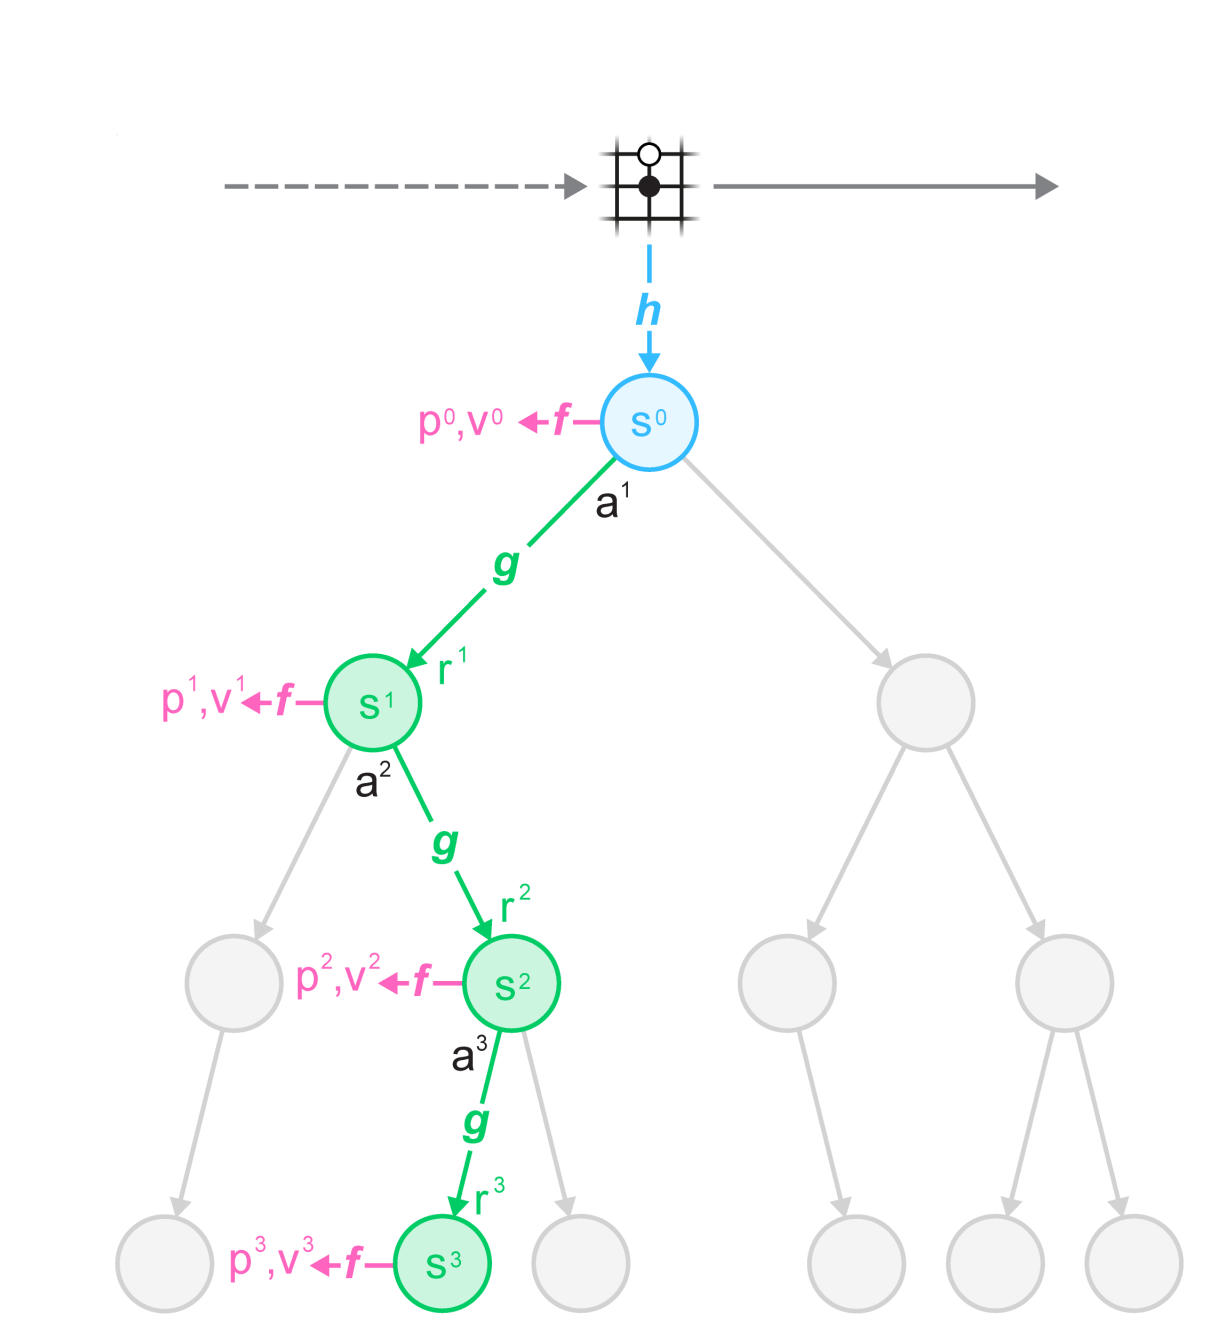
\includegraphics[height=8cm]{muzero}
    \caption{Visual representation of how the \textit{MuZero} algorithm plans ahead. \cite{muzero}}
    \label{fig:muzero}
\end{figure}

\textit{MuZero} has achieved state of the art performance across 57 Atari games and also slightly exceeded the performance of its predecessor \textit{AlphaZero} in the complex board game \textit{Go}.

\subsection{Artificial curiosity}
Artificial curiosity, in the context of reinforcement learning, describes a form of intrinsic motivation of an agent that rewards exploring the environment efficiently \cite{curious}. In contrast, algorithms without this intrinsic motivation, such as the basic \textit{$\epsilon$-greedy} strategy, may only explore randomly and with little variation from the current greedy policy, which is susceptible to local minima \cite{sutton}. This intrinsic motivation is especially useful in environments where the rewards are sparse \cite{curious}.

Several approaches exist to defining intrinsic reward functions that work well in different scenarios. For example, one may measure the distance of the current state to often visited states in order to determine how valuable the new exploration is expected to be. A different technique is called \textit{Random Network Distillation} (RND) in which the environment state is passed into a small, random neural network. As the structure of the network is unknown, the agent can only predict the network outputs well for commonly visited states, or those which are similar. Accordingly, the unpredictability of the network outputs can act as a reward signal. \cite{curious}

For model-based reinforcement learning in particular, it is possible to use the prediction error of the agent's model for a state-action pair to encourage the discovery of areas within the environment where the training effect is large. \cite{curious}

\section{Scientific goal}
The usefulness of the \textit{MuZero} algorithm combined with an intrinsic reward signal based on the \textit{dynamics} function's prediction error is tested on an agent controlling a robotic arm which is extrinsically rewarded for stacking cubes on a surface. This is a benchmark that is somewhat representative of what may be required from an agent in the field of robotics, namely, its ability to deal with large state-action spaces and sparse rewards. The experiment is simulated using the \textit{MuJoCo} \cite{gym} physics engine in a modified version of the \textit{OpenAI Gym} \cite{gym} environments for robotics.

Because the environment has a continuous action space, it must either be discretized into a potentially large amount of individual actions or the \textit{MuZero} algorithm must be further modified to allow continuous actions.

As a reference, the proposed architecture is compared with three additional agents:
\begin{enumerate}
    \item \textit{MuZero} with only the external reward signal,
    \item a model-free reinforcement learning agent with artificial curiosity, e.g. \textit{Asynchronous Advantage Actor Critic} (A3C) \cite{a3c} combined with an intrinsic reward like RND,
    \item A3C training with only the environment's external reward signal.
\end{enumerate}
However, all agents are viewed as opaque algorithms and their internal structure is ignored, meaning environment models are not trained in advance to avoid unfair advantages.

The architecture involving \textit{MuZero} and an intrinsic reward is expected to converge the fastest and achieve higher overall performance resulting from the ability to predict future states and plan ahead as well as denser rewards. Planning ahead should be especially useful in environments with large sensorimotor delays.

\section{Schedule}

\begin{figure}[h]
    \centering
    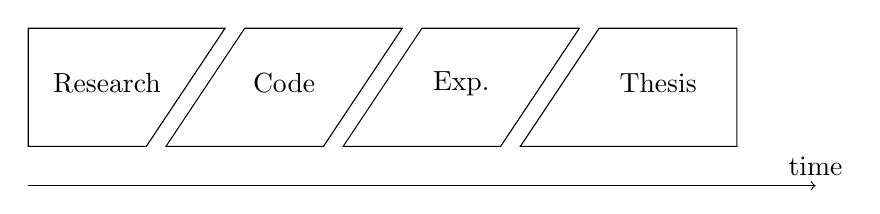
\begin{tikzpicture}
        \draw (0,0.5) -- (1.5,0.5) -- (2.5,2) -- (0,2) -- cycle;
        \node at (1.0, 1.3) {Research};

        \draw (1.75,0.5) -- (3.75,0.5) -- (4.75,2) -- (2.75,2) -- cycle;
        \node at (3.25, 1.3) {Code};

        \draw (4.0,0.5) -- (6.0,0.5) -- (7.0,2) -- (5.0,2) -- cycle;
        \node at (5.5, 1.3) {Exp.};

        \draw (6.25,0.5) -- (9.0,0.5) -- (9.0,2) -- (7.25,2) -- cycle;
        \node at (8.0, 1.3) {Thesis};
        
        \draw[->] (0,0) -- (10,0) node[anchor=south] {time};
    \end{tikzpicture}
    \caption{Planned schedule: Research, implementation, experimentation, thesis writing.}
    \label{fig:schedule}
\end{figure}

I will first perform research to fully understand model-based reinforcement learning, \textit{MuZero} in particular, and intrinsic rewards. This will ideally create a solid foundation of references for the final thesis.

The next step is to create a reference implementation using Python and TensorFlow of the \textit{MuZero} algorithm so it can be used in the experiments. The environments as well as a potential model-free agent with an intrinsic reward must also be constructed. Implementations of A3C are available.

Experiments will be performed during and after the development of the agents, starting off with simple environments to more easily test for implementation errors.

A detailed explanation of model-based reinforcement learning, artificial curiosity, \textit{MuZero} as well as the results of the experiments will then included in the final bachelor thesis.


\bibliography{bibliography}
\bibliographystyle{plain}

\end{document}
